\chapter{初段ミューオントリガーシステム}
本章では、ATLAS トリガーシステムの一つである初段ミューオントリガーシステムに着目し、Run-3 におけるエンドキャプ部初段ミューオントリガーシステムについて述べる。

\section{エンドキャプ部初段ミューオントリガー}
ATLAS 検出器でのミューオントリガーに用いる検出器は、図\ref{fig:muon}に示すように RPC を用いるバレル部と TGC を用いるエンドキャップ部に分かれている。以下では TGC を用いるエンドキャップ部でのトリガーシステムについて説明する。エンドキャプ部はさらに2つの領域に分けられ、$1.05 < |\eta| < 1.9$ をエンドキャップ領域、$1.9 < |\eta| < 2.4$ をフォワード領域と呼ぶ。
\begin{figure}[tb]
  \centering
  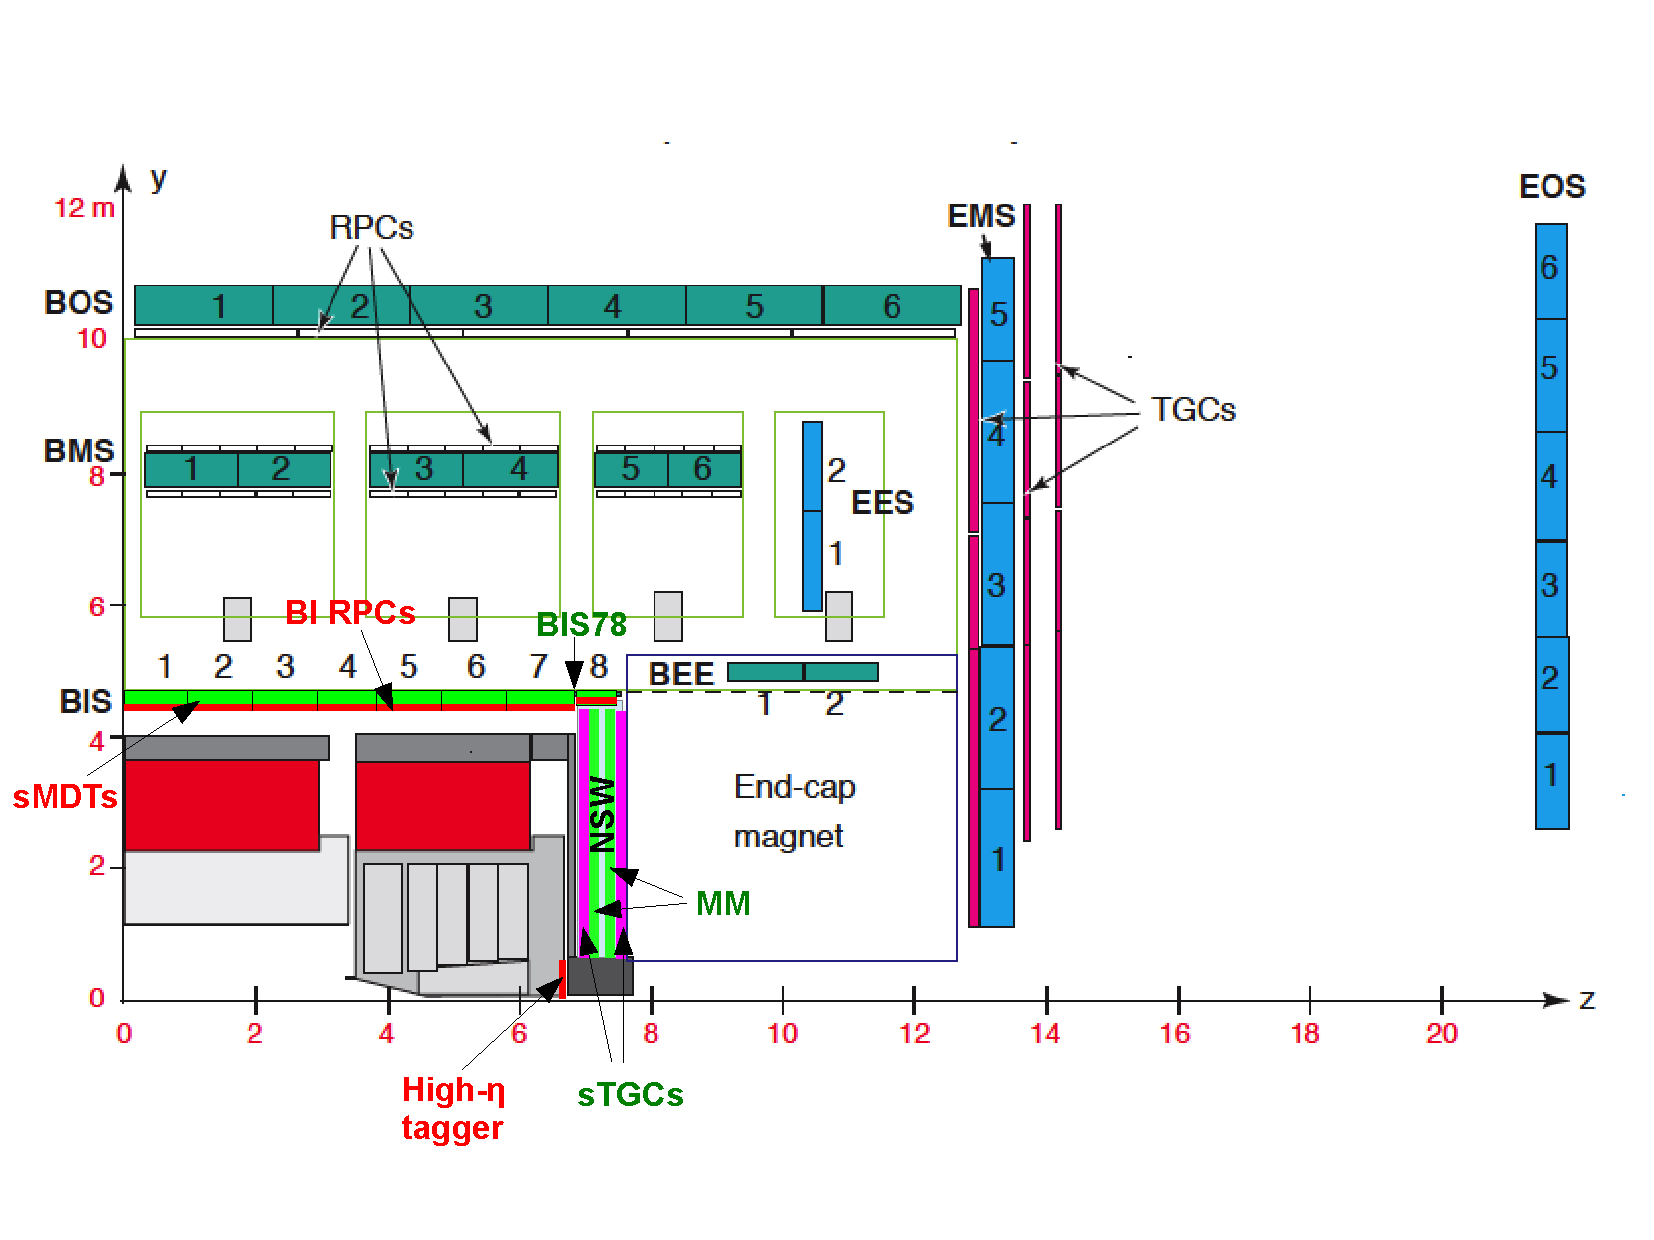
\includegraphics[clip, width=14cm]{fig/2/ch01_fig_03a.pdf}
  \caption{初段ミューオントリガーに用いる検出器の設置位置。}
  \label{fig:muon}
\end{figure}

\subsection{エンドキャップ部ミューオントリガーの概要}\label{section:CW}
エンドキャップ部初段ミューオントリガーで用いられるトリガー判定の概要を図\ref{fig:trigger-scheme}に示す。
衝突点で生成されたミューオンはトロイド磁石の磁場領域より内側にある検出器を通過した後、トロイド磁場領域を通り TGC に到達する。トロイド磁石による磁場は $\phi$ 方向にかかっているため、ミューオンの飛跡はトロイド磁場中で$\eta$ 方向に曲げられる。さらに、衝突点付近のソレノイド磁石で生じる $z$ 方向の磁場成分と、トロイド磁石付近で生じた $R$ 方向の磁場成分によって、ミューオンの飛跡は $\phi$ 方向にも曲げられる。ミューオンの飛跡の曲がり具合は 横方向運動量$p_T$ の大きさによって変化するため、飛跡情報からミューオンの$p_T$を算出することができ、トリガー判定に使用することができる。

トロイド磁場によって曲げられたミューオンは TGC BW の M1, M2, M3 にヒットを残す。ここで、衝突点と M3 のヒット位置を結んだ直線をミューオンが無限運動量で通過したと仮定した場合の飛跡として扱う。この無限運動量を持つミューオンの飛跡と磁場によって曲げられた実際の飛跡を比較し、M1 におけるヒット位置の $R$ 方向と $\phi$ 方向のずれ $dR$、$d\phi$ を計算する。
そして、あらかじめ $dR$、$d\phi$ に対応する $p_T$ を Look-Up Table (LUT) として作成しておき、参照する事で短時間で $p_T$ を出力を可能としている。

\begin{figure}[tb]
  \centering
  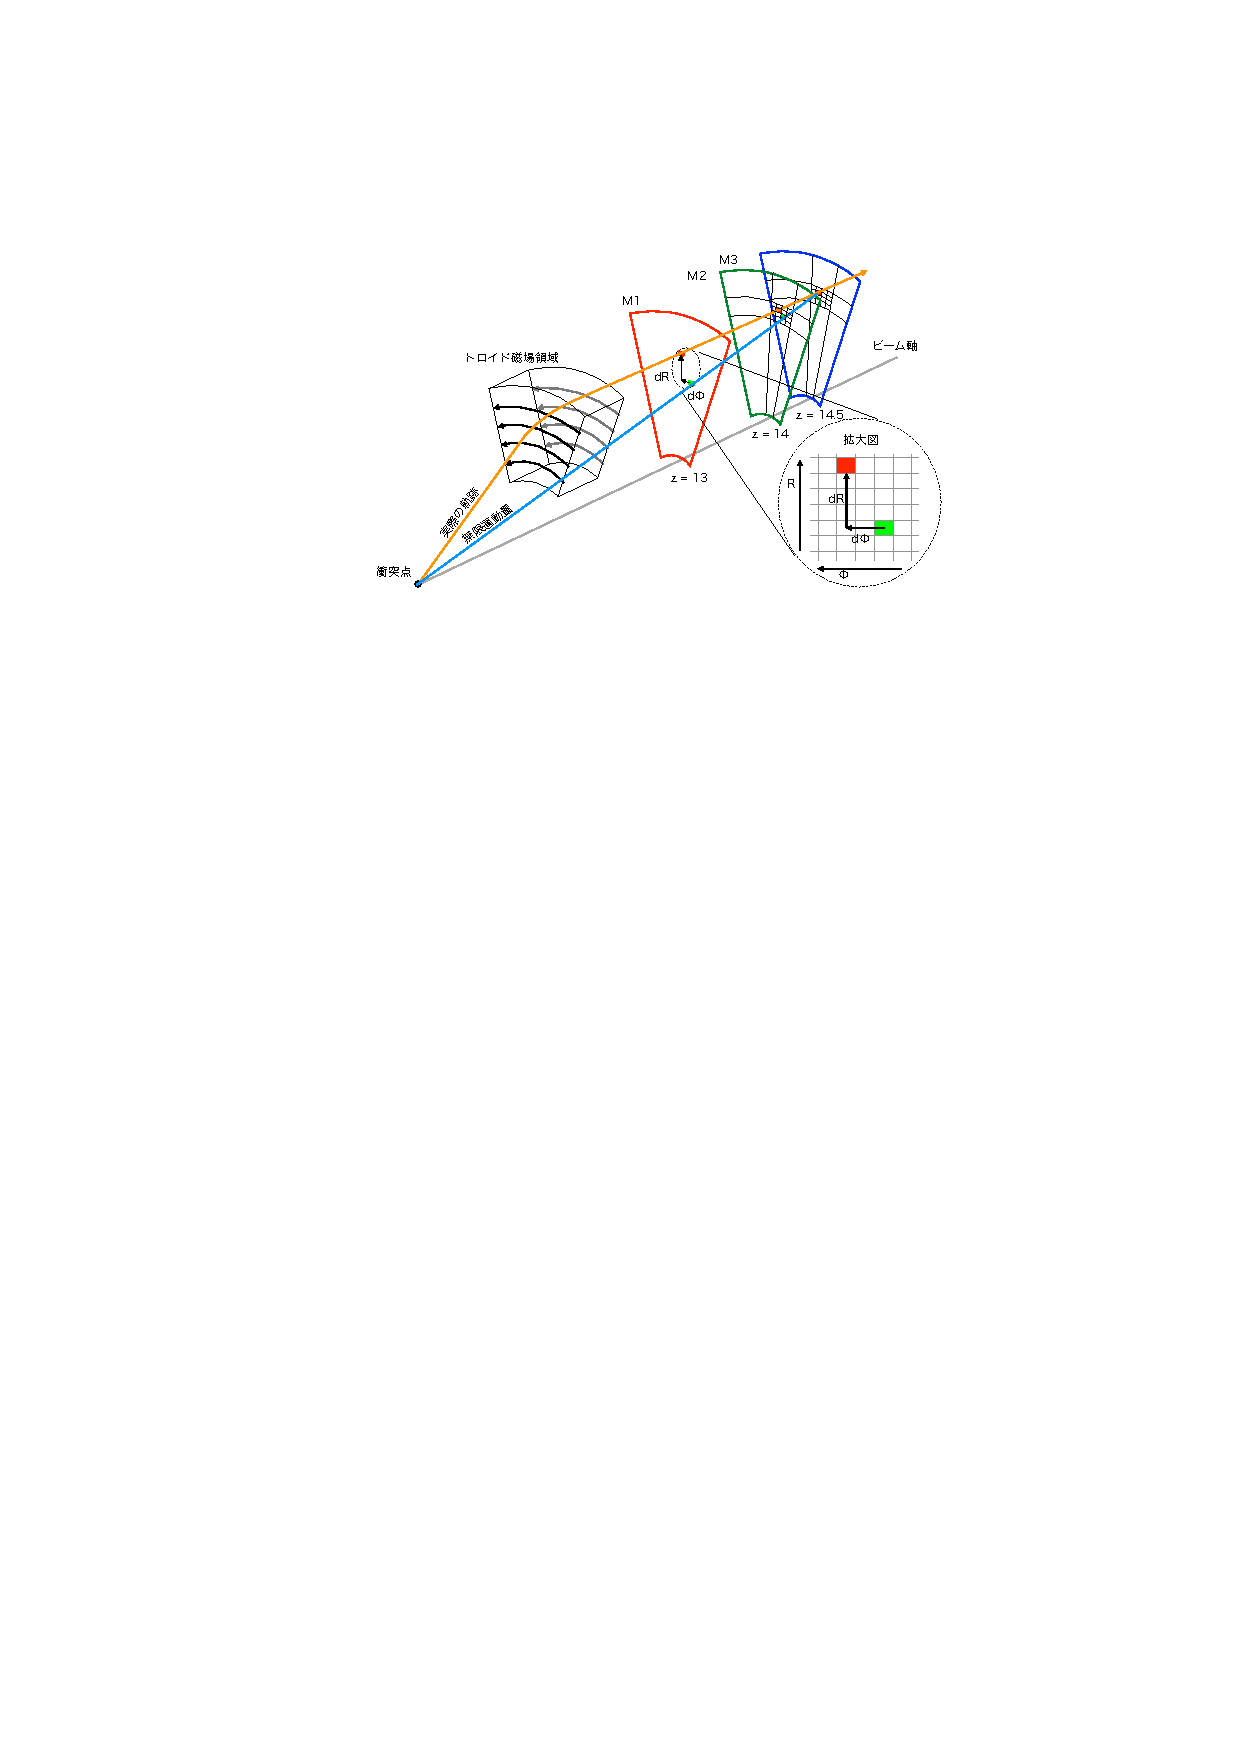
\includegraphics[clip, width=15cm]{fig/3/akatsuka_mt_trigger_scheme.pdf}
  \caption{ATLAS検出器エンドキャップ領域におけるトリガースキームの概念図\cite{article:akatsuka-mron}。無限大の運動量を持つミューオンを仮定し、磁場によって曲げられたミューオンとの位置の差を用いて$p_T$を計算する。}
  \label{fig:trigger-scheme}
\end{figure}

LUT とは入力データに対応する出力データを参照するための表のことを指し、$dR$、$d\phi$ を入力として $p_T$ を出力する LUT を FPGA に保存している。
この LUT は Coincidence Window (CW) と呼ばれており、あらかじめ MC サンプルや実際の測定データを用いて$dR$、$d\phi$に対応する $p_T$ を算出し、図\ref{fig:CW}のような形で保存されている。
エンドキャップ部のトロイド磁場や TGC は理想的には 8 回対称だが、磁場の向きや TGC チェンバーの設置位置のずれなどがあるため、CW は TGC BW のすべてのトリガー判定を行う位置ごとに作成されている。
Run-3 で使用される CW は図\ref{fig:CW}のように 15 個に分類されている。この各色が 15 段階の $p_T$ 閾値に対応しており、各 $p_T$ 閾値に付された符号はミューオンの電荷に対応している。図\ref{fig:CW}のマスの中の数字は表\ref{pt_number} に示す pt number と対応している。

\begin{figure}[tb]
  \centering
  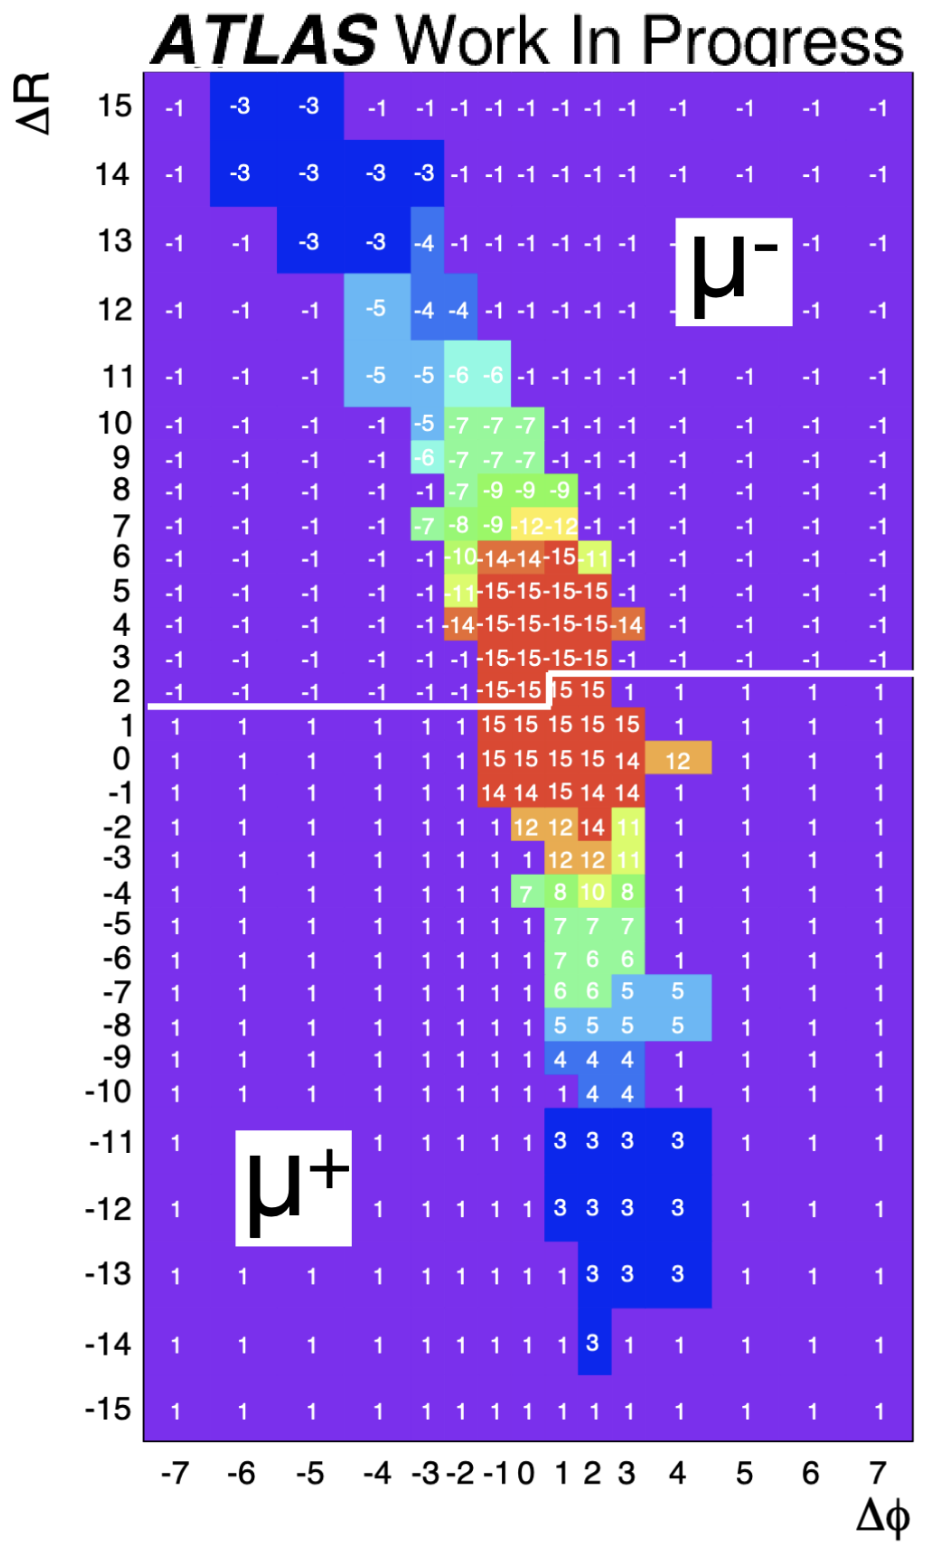
\includegraphics[clip, width=7cm]{fig/3/cw_run3_shiomi.png}
  \caption{Run-3 での TGC における Coincidence Window の例。ミューオンのヒットがあった時にそれぞれの検出位置のの CW を参照し、$dR$、$dφ$ からミューオンの $p_T$ を 15 段階で見積もる。}
  \label{fig:CW}
\end{figure}

\begin{table}[tb]
    \caption{Run-3 初段ミューオントリガーにおける 15 段階の $p_T$ の値。}
    \label{pt_number}
    \centering
    \begin{tabular}{|c|c|c|c|c|c|c|c|c|c|c|c|c|c|c|c|c|c|c|c|c|c|c|c|}
        \hline
        $p_t$ number & 1 & 2 & 3 & 4 & 5 & 6 & 7 & 8 & 9 & 10 & 11 & 12 & 13 & 14 & 15\\
        \hline
        $p_T$ [GeV] & 3 & 4 & 5 & 6 & 7 & 8 & 9 & 10 & 11 & 12 & 13 & 14 & 15 & 18 & 20\\
        \hline
    \end{tabular}
\end{table}

\subsubsection{トリガーセクター}
TGC のトリガー判定に用いられる単位の模式図を図\ref{fig:RoI}に示す。TGC のトリガー判定はトリガーセクターごとに行われ、領域内のミューオンの情報から判定結果が出される。
エンドキャップ部のトリガーセクターは、 $\phi$ 方向にエンドキャプ領域では 48 個、フォワード領域では 24 個に分割している。
これらのトリガーセクターはさらに小さな領域である Region of Interest (RoI) に分割される。
図\ref{fig:RoI} に示すように、エンドキャップ領域のトリガーセクターは $\eta$ 方向に 37 分割、$\phi$ 方向に 4 分割されるため 148 個の RoI で構成されている。フォワード領域のトリガーセクターは $\eta$ 方向に 16 分割、$\phi$ 方向に 4 分割されるため 64 個の RoI で構成されている。また RoI を $\eta$ 方向に 2 つ、$\phi$ 方向に 4 つまとめたものを Sub Sector Cluster (SSC) と呼ぶ。RoI は TGC の持つミューオンの検出位置情報の最小単位であり、$p_T$ 判定に用いる CW はこの RoI ごとに作成している。

\begin{figure}[tb]
  \centering
  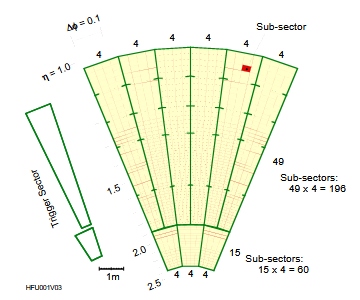
\includegraphics[clip, width=10cm]{fig/3/RoI.png}
  \caption{TGC におけるトリガーセクターと RoI の模式図。緑の線で囲まれた領域が 1 つのトリガーセクターを表し、赤の線で囲まれたマスが 1 つの RoI を表す。}
  \label{fig:RoI}
\end{figure}

\subsection{初段ミューオントリガーにおけるエレクトロニクス}
初段ミューオントリガーでは、ATLAS 検出器から送られてくる情報に対して SectorLogic、MUCTPI、L1Topo、CTP という電子回路を経てトリガーが発行される。
以下では各エレクトロニクスについて説明する。

\subsubsection{Amplifier Shaper Discriminator (ASD) ボード}
Amplifier Shaper Discriminator (ASD) ボードは TGC のワイヤーとストリップからアナログ信号を受け取り、デジタル信号への変換を行う。
ASD ボード上の ASD において TGC からのアナログ信号を増幅・整形し、 閾値電圧を超えた信号のみ LVDS 信号として出力される。1 枚の ASD ボードは 4 つの ASD ASIC を搭載しており、ASD ASIC は 4 つの信号の受信・処理を行う。そのため、同時に 16 チャンネルの信号を処理することが可能である。

\subsubsection{Patch-Panel ASIC (PP ASIC)}
Patch-Panel ASIC は ASD からワイヤーとストリップそれぞれの LVDS 信号を受け取り、タイミングの調整を行うことで、同じ陽子衝突由来の信号を同時に次の SLB ASIC に送る。陽子衝突が起きてからミューオンが検出器に到達する時間や、ケーブルの長さの違いにより、信号のタイミングが各チャンネルごとに異なるため、PP ASIC を用いてタイミングの調整を行う。

\subsubsection{Slave Board ASIC (SLB ASIC)}
Slave Board ASIC は読み出しとトリガー判定の 2 種類の処理を行う。
トリガー判定で行う処理としては、各チャンネルの情報を用いてコインシデンスを取ることである。
TGC Triplet (M1 ステーション) ではワイヤーの場合は 3 層中 2 層にヒットがあることを要求し、ストリップの場合は 2 層中 1 層にヒットがあることを要求する。
2 つの TGC Doublet (M2、M3 ステーション) では、各ステーションから信号を受け取りワイヤーとストリップで独立に 4 層中 3 層以上にヒットがあることを要求する。 これらのコインシデンス結果はLVDS 信号で後段の High PT ボードに送る。

\subsubsection{High PT (HPT) ボード}
High PT ボードは、M1 の SLB と M2,M3 の SLB からのコインシデンス結果を受け取り、 M1,M2,M3 の 3つのステーション間のコインシデンスを行う。M1 と M3 の位置情報から ($\Delta R$, $\Delta \phi$) を計算し、次の Sector Logic に送る。Sector Logic にはボードごとに、位置情報 $R$ と $\phi$ 、位置の差の情報 $\Delta R$ と $\Delta \phi$ を G-Link 通信を用いて送信する。データ通信速度の制限により、1 つの HPT ASIC から最大 2 候補を選んで送信している。

\subsubsection{New Sector Logic (NSL)}
New Sector Logic では TGC-BW とトロイド磁石の内側にある検出器の情報を統合してトリガー判定を行う。
TGC-BW の HPT ボードからは、ミューオン候補の情報が G-Link 規格で送られてくる。
RPC BIS78、Tile カロリメータ、 TGC-EI からは、検出器におけるヒット情報が送られてくる。
NSW からは通過したミューオンの飛跡情報が送られてくる。
NSL はこれらの情報をもとにトリガー判定を行い、トリガー判定の結果を MUCTPI に送信する。

NSL ボードでは、 HPT ボードから受け取った TGC BW の位置情報 $R$ と $\phi$ 、位置の差の情報 $\Delta R$ と $\Delta \phi$ を用いて $p_T$ の判定を行う。各 ($R$, $\phi$) からミューオンのヒット位置を表す RoI を決定し、($\Delta R$, $\Delta \phi$) から NSL 上に実装されている Coincidence Window を用いて $p_T$ に変換する。






\section{2022年 Run-3 における初段ミューオントリガーの性能}
本節では2022年 Run-3 で使用されている CW のトリガー性能について述べる。

\subsection{解析手法}
実際の実験データはトリガーによって選別された粒子の情報のみが保存されているため、そのままのデータを用いてトリガーの性能評価や解析を行うとバイアスがかかる可能性がある。そこで解析の手法として Tag$\&$Probe 法を用いる。

本研究では、内部飛跡検出器とミューオン検出器でそれぞれ独立に再構成され、その後飛跡が結合できたZ ボソン由来のミューオン候補を用いて評価を行う。1回の衝突事象に対し、2 つ以上のミューオン候補が存在するイベントのみを用いる。それらのミューオン候補のうち、任意の2つの電荷が異符号となっているミューオンペアを選び出し、不変質量を再構成する。再構成の条件は、$80 GeV < M_Z < 100 GeV$ とする。
これらのミューオンのうち、一方を Tag ミューオン、もう一方を Probe ミューオンと定義する。
まず、Tag ミューオンがトリガーを発行したかどうかを判定する。Run-2 での実験データを解析に使用する際のトリガー判定には、HLT のシングルミューオントリガーである 「HLT$\_$mu26$\_$ivarmeduium」 を使用する。
ここでトリガー発行の判定を行うために $\Delta R = \sqrt{(\Delta \eta)2 + (\Delta \phi)2}$ を定義する。ここで $\Delta \eta$, $\Delta \phi$ はそれぞれデータの保存されているトリガーを発行した飛跡と Tag ミューオンの $\eta$ 方向、$\phi$ 方向の差である。図\ref{fig:tag_HLT}にTag ミューオンと HLT の $\Delta R$ 分布を示す。本研究では$\Delta R < 0.001$ を満たせば Tag ミューオンがトリガーを発行したとみなす。Tag ミューオンが HLT を発行しているとみなされた時、もう一つのミューオンを Probe ミューオンとして解析に使用する。

\begin{figure}[tb]
  \centering
  \rule{8cm}{6cm}
  \caption{Tag ミューオンと HLT の $\Delta R$ 分布。$\Delta R < 0.001$ ならば Tag ミューオンが HLT を発行したものとする。}
  \label{fig:tag_HLT}
\end{figure}

Probe ミューオンは正しく再構成され、発行されたトリガーとは独立なミューオンである。
Probe ミューオンを使用してエンドキャプ部のトリガー性能を評価するために、Probe ミューオンと TGC のヒット情報を一致させる。図\ref{fig:Probe_TGC}に Probe ミューオンと TGC のヒット情報 の $\Delta R$ 分布を示す。本研究では$\Delta R < 0.04$ を満たせば Probe ミューオンが TGC のヒット情報と一致したものとする。
Probe ミューオンの情報とこのミューオンと一致したTGC のヒット情報を使って解析を行う。

\begin{figure}[tb]
  \centering
  \rule{8cm}{6cm}
  \caption{Probe ミューオンと TGC のヒット情報との $\Delta R$ 分布。$\Delta R < 0.005$ ならば Probe ミューオンが TGC のヒット情報と一致したものとする。}
  \label{fig:Probe_TGC}
\end{figure}



\subsection{トリガーの効率の算出}
トリガー効率$\epsilon$について式\ref{equ:Eff}を用いて評価を行う。
ここで、全ミューオン数はTGC にヒットした全オフラインミューオンと定義し、その中でトリガーを発行したミューオンの数を調べ、トリガー効率を計算する。
このとき得られるトリガー効率を $p_T$ の関数で表したプロットを Turn-on curve と呼ぶ。
\begin{equation}
 \epsilon=\frac{トリガーを発行したミューオンの数}{全ミューオンの数}
 \label{equ:Eff}
\end{equation}
シングルミューオンのシミュレーションサンプルに対してトリガー効率を計算し、2022年Run-3 で使用されているトリガーの各閾値における Turn-on curve を図\ref{fig:Run3_15_MC}に示す。
\begin{figure}[tb]
  \centering
  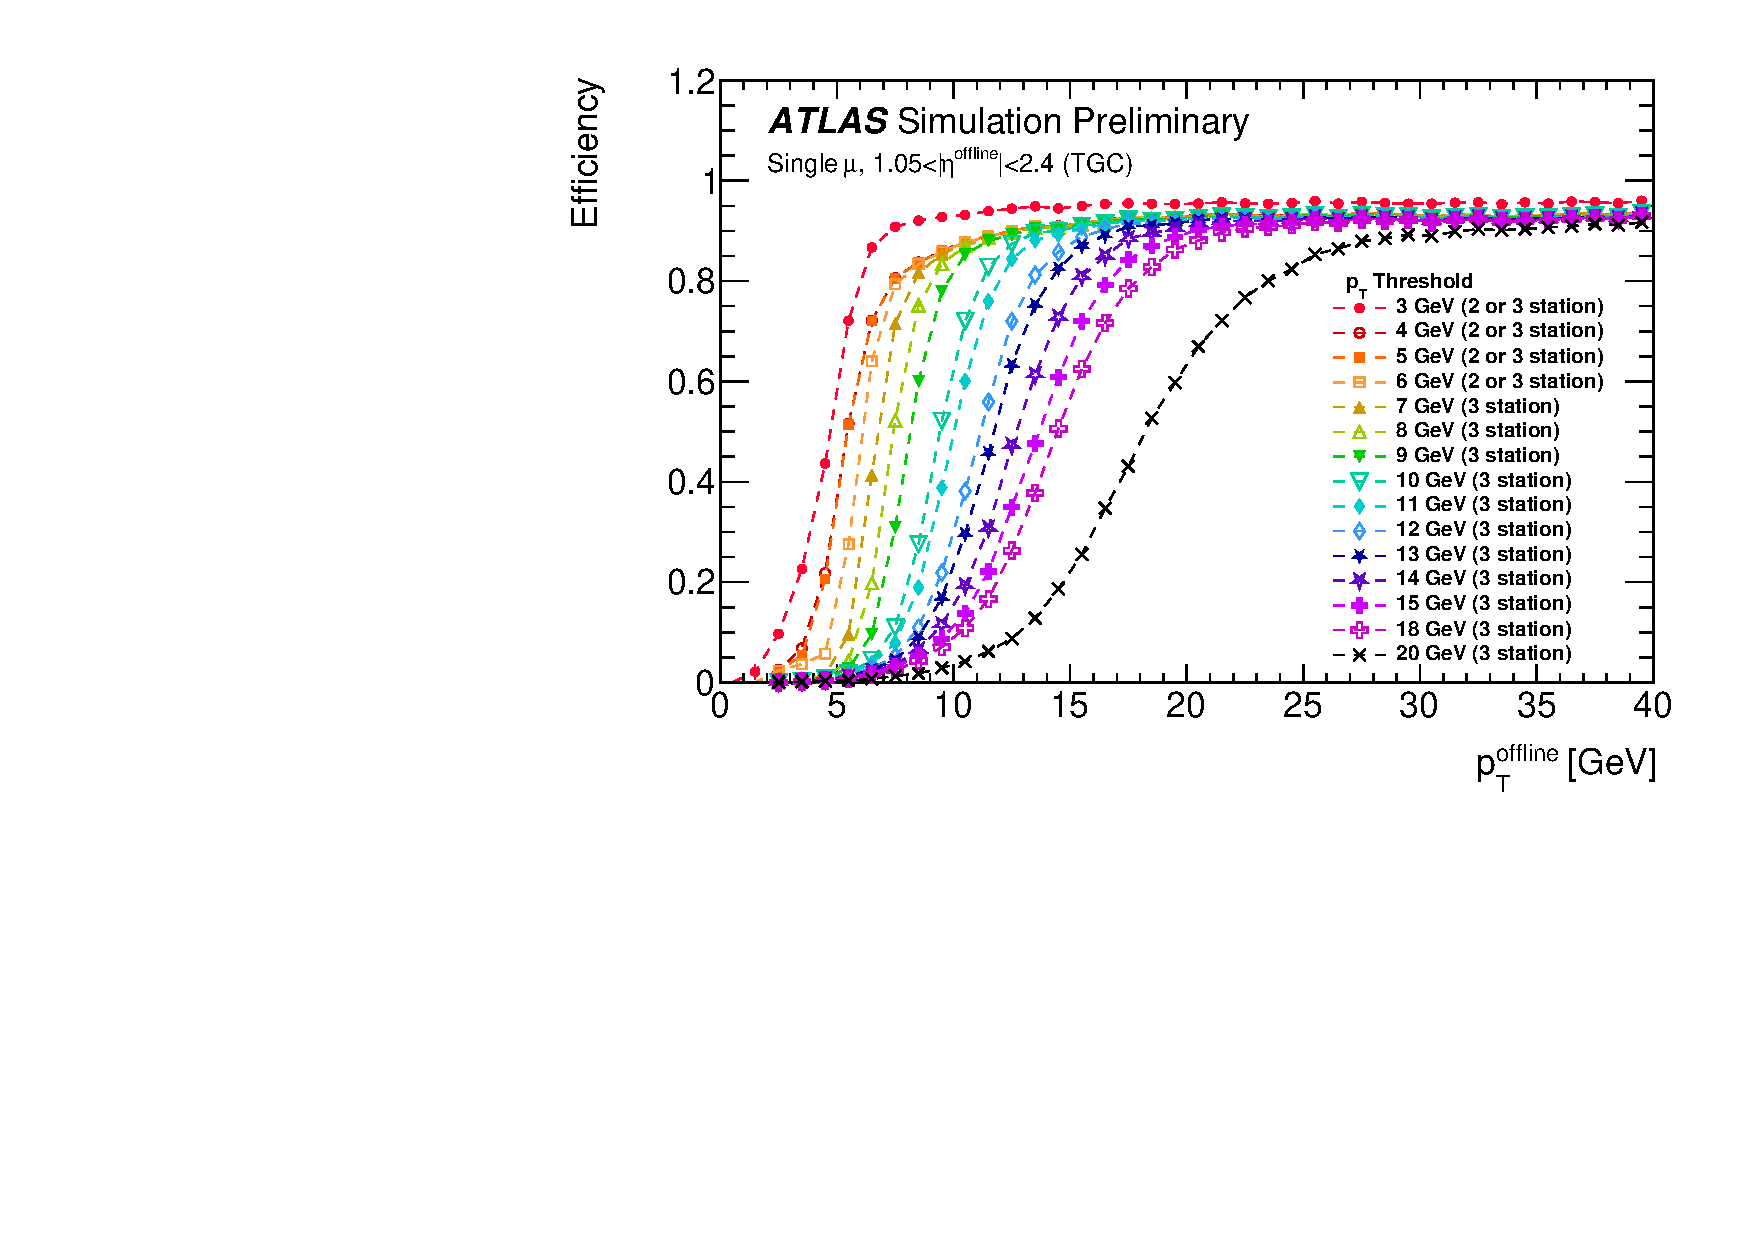
\includegraphics[clip, width=15cm]{fig/3/PLOT-TRIG-2020-01-fig1.pdf}
  \caption{Run-3 における15段階閾値のTurn-on curve。シングルミューオンのシミュレーションサンプルに対してのトリガー効率を示している。}
  \label{fig:Run3_15_MC}
\end{figure}
また、Run-3 の実データに対してトリガー効率を計算し、各閾値におけるトリガー効率を pT の関数として表した結果を図\ref{fig:Run3_15_Data}に示す。
\begin{figure}[tb]
  \centering
  \rule{8cm}{6cm}
  \caption{Run-3 における15段階閾値のTurn-on curve。Run-3 の実データに対してのトリガー効率を示している。}
  \label{fig:Run3_15_Data}
\end{figure}
さらに、各チェンバーごとの各閾値におけるトリガー効率を図\ref{fig:Run3_15_Data_chamber1}に示す。
\begin{figure}
    \centering
    \begin{minipage}[b]{0.4\linewidth}
        \centering
        %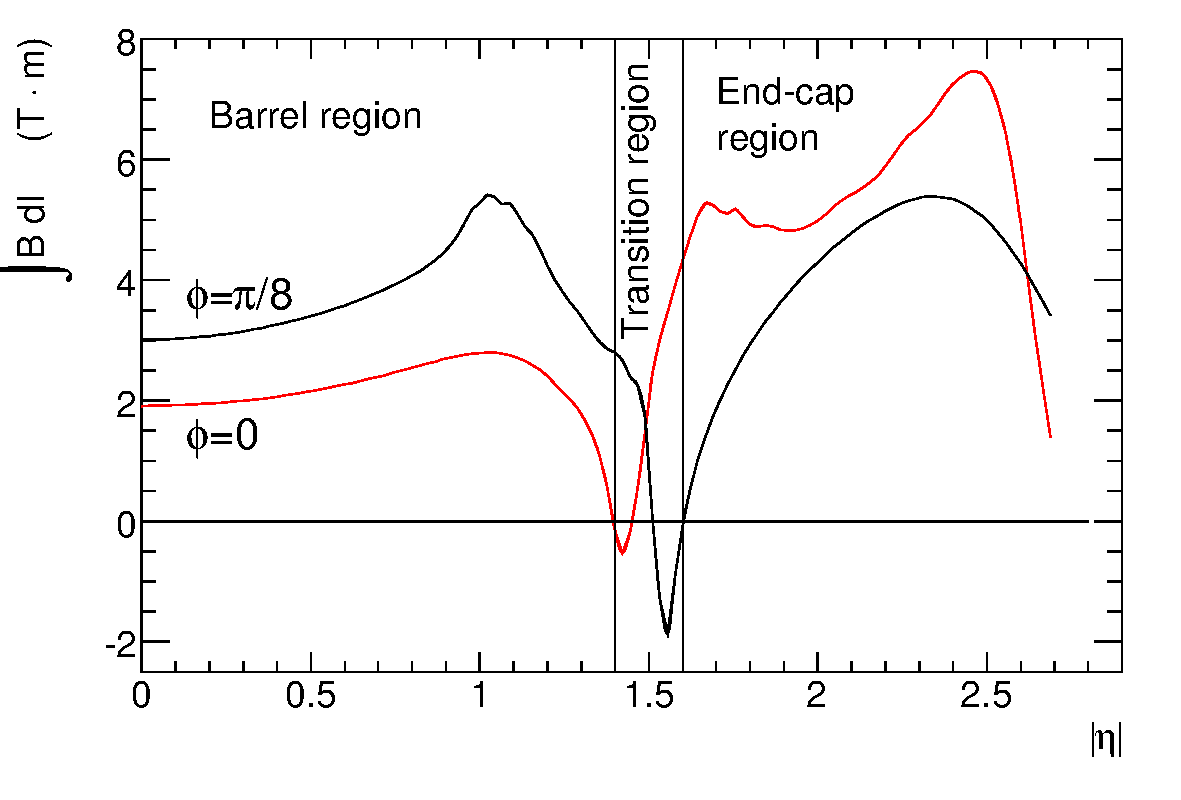
\includegraphics[clip, width=7cm]{fig/2/IBdl.pdf}
        \rule{6cm}{4cm}
        \vspace{10pt}
        \subcaption{}
        \label{}
    \end{minipage}
    \hfill
    \begin{minipage}[b]{0.4\linewidth}
        \centering
        %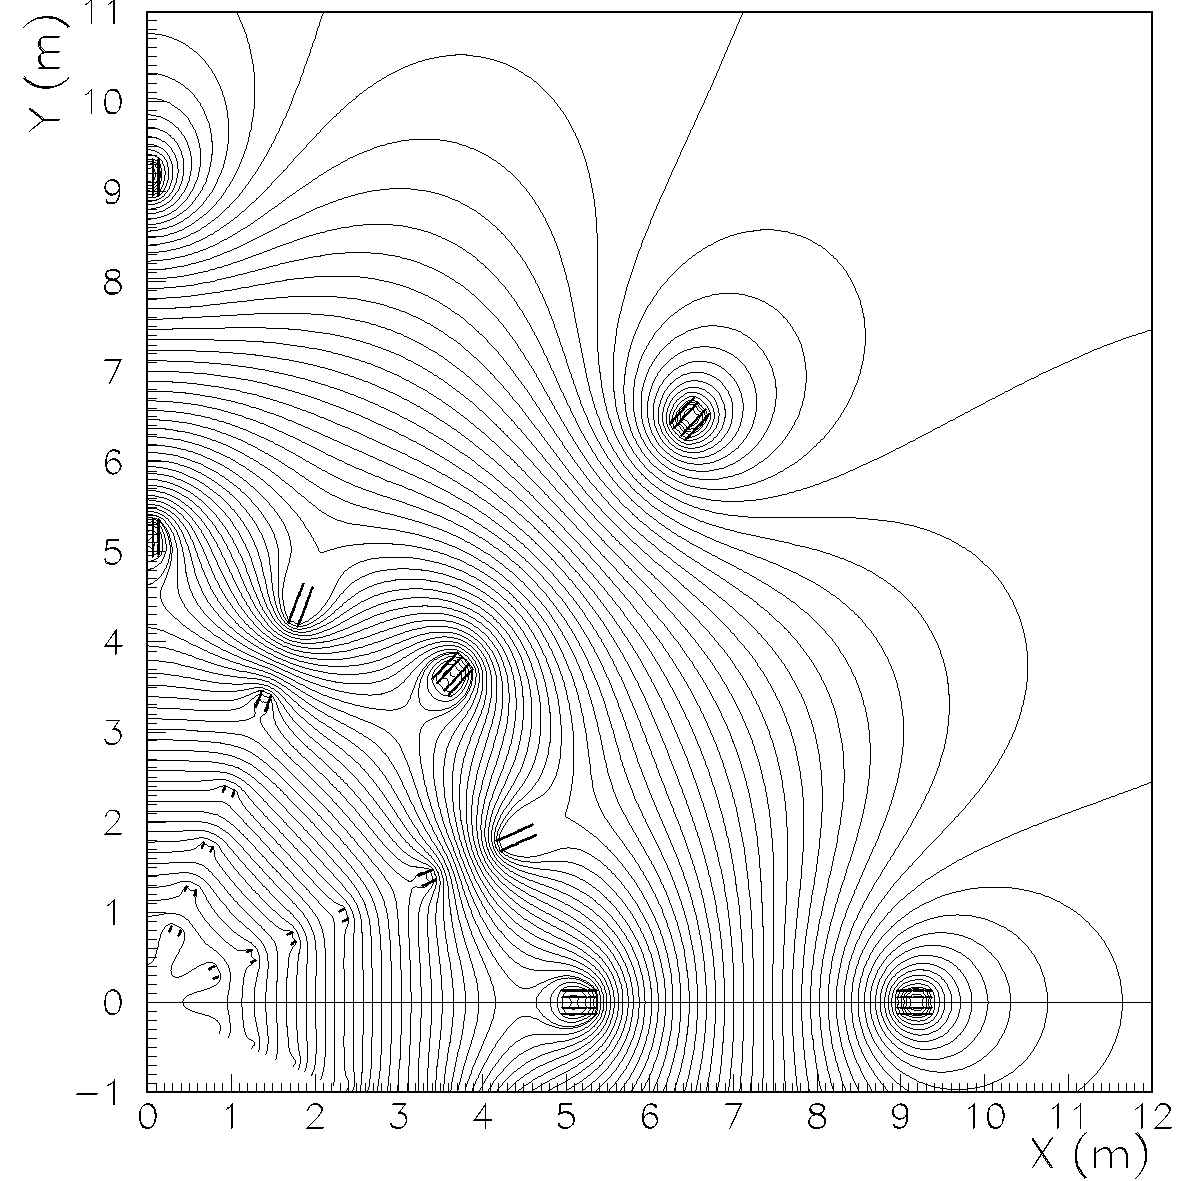
\includegraphics[clip, width=6cm]{fig/2/FMBmap.pdf}
        \rule{6cm}{4cm}
        \vspace{10pt}
        \subcaption{}
        \label{}
    \end{minipage}
    \caption{Run-3 における15段階閾値のTurn-on curve。Run-3 の実データに対しての各チェンバーごとトリガー効率を示している。(1-48個作る)}
    \label{fig:Run3_15_Data_chamber1}
\end{figure}

定量的な評価を行うために、式\ref{equ:fitting}を用いて Turn-on curve にフィッティングを行う。
\begin{equation}
    f(p_T) = \frac{p_0}{exp(\frac{p_T-p_1}{p_2})+1}
 \label{equ:fitting}
\end{equation}
ここで、トリガーの性能を表す 3 つのパラメータ $p_0$, $p_1$, $p_2$ を以下のように定義する。
\begin{enumerate}\label{table:fitting}
   \item $p_0$:Plateau efficiency\\
   Turn-on curve が横這いになった時のトリガー効率を表す。トリガー閾値以上の pT を持つミューオンに対するトリガー効率を表すため、その値が 1 に近い方が高性能である。
   \item $p_1$:Effective threshold\\
   トリガーの実効的な $p_T$ の閾値を表す。トリガー効率が Plateau efficiency の値の 50\% となる時の $p_T$ の値である。
   \item $p_2$:Resolution\\
   トリガーの運動量の分解能を表す。Turn-on curve の立ち上がりの鋭さに対応すしており、Resolution の値が大きくなると Turn-on curve の立ち上がりが緩くなるため、、トリガーの運動量分解能が悪くなる。
\end{enumerate}


ミューオンの電荷依存に対する評価

\begin{figure}[tb]
  \centering
  \rule{8cm}{6cm}
  \caption{電荷}
  \label{fig:fit_def}
\end{figure}



\subsection{トリガーレートの算出}
トリガーレートとは、実験データにおけるトリガーが発行された事象数である。ここでは HLT でのトリガー発行のバイアスを防ぐために、L1 Trigger のみを要求し、HLT は passthrough のトリガーである 「HLT$\_$noalg$\_$L1MU20」を要求する。 は 2016 年で取得されたデータを用いて算出したトリガーレートの $\eta$ 依存性である。

\begin{figure}[tb]
  \centering
  \rule{8cm}{6cm}
  \caption{Rate}
  \label{fig:Run3_rate}
\end{figure}

\subsection{現行のCWの問題点}
2022年 Run-3 で使用されている CW にはいくつかの問題点がある。
・電荷


・検出器アライメントを行っていないことによるEfficiencyの低下



\section{CW の最適化手法}\label{section:最適化}
Run-2 で行われたTGC 検出器の設置位置のズレや歪みを考慮した CW の最適化を行う方法について述べる。

\subsection{TGC 検出器の設置位置による影響}
シミュレーション上では TGC 検出器などの検出器は設計通りの位置に設置されている。そのため、シミュレーションサンプルを用いて作成されている CW は検出器のズレや歪みを考慮できていない。設置位置が設計位置からズレている場合、想定されていたミューオンの飛跡から外れてしうため、 CW を用いた運動量判定に影響が出てしまい、トリガーの運動量分解能の低下を招く。

TGC のアライメントのズレの測定方法はこれまでの研究で既に確立されている。
図\ref{fig:ズレ}に Run-2 での実データを用いた TGC 検出器の設置位置のズレを示す。

\begin{figure}[tb]
  \centering
  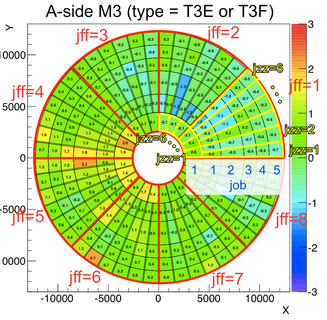
\includegraphics[clip, width=10cm]{fig/4/zure.png}
  \caption{Run-2での検出器のズレの測定図}
  \label{fig:ズレ}
\end{figure}


\subsection{検出器アライメント}
CW に対して検出器のズレを補正し最適化することで、トリガー効率を維持しつつ、トリガーレート削減を目指す。
Run-2で行われたシミュレーションを用いて作成した CW に対する TGC アライメントの補正方法について以下に述べる。


Run-2 では
2015 年 Run-2 の実データを用いた
この CW を cell 毎に判定する方法を CW optimization と呼ぶ。


・検出器アライメント
<山内さんの手法>
<木戸さんの手法の説明>


\section{本研究の目的}
CW は事前にシミュレーションデータを用いたミューオンの運動量分布から統計的に作成する。そして、実際のデータをもとに、ある運動量を持つミューオンのヒットマップを作成し、ヒットマップと CW を比較することで検出器アライメントの補正値を判断して CW の最適化を行っている。
このように従来の CW の作成から最適化までの作業では、大量のシミュレーションデータや実際のデータの傾向を CW に反映させることを手動で行っていた。
そのため、Run-3における初段ミューオントリガーの性能を向上させるためには Run-2 と同様に CW の最適化を行う必要がある。しかし、\ref{section:最適化}節で述べたような Run-2 で行われていた最適化手法は、各CWごとに1マスずつ6段階の閾値を一段階ずつ確認する手法のため膨大な作業量が必要である。そのため、Run-3 で15段階に増設された閾値を持つ CW に対して Run-2 での最適化手法を行うことは現実的でない。
そこで、本研究では近年急速に発展している機械学習に着目し、新たな CW の最適化手法の開発を行う。















